\subsubsection{\stid{1.14} UPC++\label{subsubsect:upcxx}} 
\paragraph{Overview} 

UPC++~\cite{upcxx-site} is a C++ library
supporting Partitioned Global Address Space (PGAS) programming~\cite{upcxx-ipdps19,upcxx-guide,upcxx-spec}.
The current UPC++ v1.0 (distinct from an earlier prototype designated V0.1
\cite{zheng:ipdps14}) is distinguished by three guiding principles.
First, all communication is \emph{asynchronous}, allowing overlap of computation and
communication, and encouraging programmers to avoid global synchronization. Second, all communication
is \emph{syntactically explicit}, encouraging programmers to consider the costs of communication. Third,
UPC++ encourages the use of \emph{scalable data-structures},
avoiding non-scalable library features.
These principles provide a programming model that can
scale efficiently to potentially millions of processors.
UPC++ is well-suited for implementing elaborate distributed data structures where
communication is irregular or fine-grained. 
The UPC++ communication interfaces for Remote Memory Access (RMA) 
and Remote Procedure Calls (RPC)
are composable and fit naturally within the context of modern C++.

UPC++ is needed for ECP because it delivers low-overhead communication,
efficiently embracing PGAS support offered by modern systems,
such as Remote Direct Memory Access (RDMA) offload capabilities of modern
network hardware and native on-chip communication between distinct address
spaces.  
UPC++'s low-overhead communication mechanisms can maximize injection rate and
network utilization, tolerate latency through overlap, streamline unpredictable
communication events, minimize synchronization, leverage hardware support for
communication involving accelerator memory, and efficiently support small- to
medium-sized messages arising in many applications.
The importance of these properties is reinforced by application trends; many
ECP applications require the use of irregular data structures such as adaptive
meshes, sparse matrices, particles, or similar techniques, and also perform
dynamic load balancing.
Because of such trends, the UPC++ library provides an essential ingredient for
the ECP software stack; enabling it to exploit the best-available communication
mechanisms, including novel features being developed by vendors.  UPC++
provides seamless and efficient multithreading support, offering a
complementary and interoperable approach to ``MPI + X'', enabling developers to
focus their effort on optimizing performance-critical communication.

\paragraph{Key Challenges}

As a result of technological trends, the cost of data motion is steadily increasing relative to that of computation.  To reduce communication costs, we need to 
reduce the software overheads and hide communication latency behind available computation. UPC++ addresses both strategies.
UPC++ avoids the software overheads associated with MPI, 
instead relying on the GASNet-EX~\cite{gasnet-site,gasnet-lcpc18}
communication library which is specifically designed and tuned
for native PGAS communication using the best-available hardware
mechanisms on each network
(see Section~\ref{subsubsect:gasnet-ex} on GASNet-EX, which is being co-designed).
UPC++ supports asynchronous communication via one-sided RMA and RPC.

\paragraph{Solution Strategy}

The UPC++ project has two primary thrusts:

% Non-use of a enumerated environment is intentional, due to excessive whitespce

\textbf{1. Increased performance through reduced communication costs:} 
%The UPC++ programmer can expect communication to run at close to hardware speeds.
UPC++ leverages the underlying GASNet-EX communication library to deliver efficient, low-overhead RMA and RPC on HPC systems.
This includes accelerated transfers to and from GPU memory.
UPC++ features encourage aggressively asynchronous execution,
enabling applications to overlap the latency of communication with
available computation or additional communication.

\textbf{2. Improved productivity:} UPC++'s treatment of asynchronous
execution utilizes futures and promises, which simplify the management of
asynchrony.
The \texttt{upcxx::copy} API provides concise expression of RMA involving any
combination of shared host and GPU memory, without the need for the application
to stage GPU data through host memory buffers.

The PGAS model and one-sided RMA communication offered by UPC++
benefit application performance by mapping tightly onto the RDMA mechanisms
supported by the network hardware. GASNet-EX provides the
thin middleware needed to implement RMA efficiently on a variety of platforms,
from laptops to supercomputers.
One-sided communication provides an additional benefit of
decoupling synchronization from data motion,
avoiding the fine-grained synchronization overheads of message passing.

UPC++'s Remote Procedure Call (RPC)
enables the programmer
to easily execute code on remote processes.
RPC is useful in managing access to complicated irregular data structures,
and in expressing asynchronous task execution, where communication patterns
are data-dependent and hence difficult to predict.

As one example of how our approach is applicable to real application kernels,
we modified a GPU-enabled 3D heat conduction example from a Kokkos tutorial to
convert the inter-node communication from MPI message passing to UPC++
RMA~\cite{pawatm21-upcxx-kokkos}.  The primary goal of this study was to
demonstrate that comparable programming effort with UPC++ and MPI could yield
comparable performance. However the finding was that with both versions written
na\"{\i}vely, the UPC++ RMA version gave measurably superior performance.
Figure~\ref{fig:paw21_interop_strong_scaling} shows a strong scaling study on
OLCF's Summit, comparing performance using 
CUDA-aware IBM Spectrum MPI versus UPC++ with the CUDA memory kind.

\begin{figure}[htb]
  \centering
  \captionsetup{width=0.85\linewidth}
  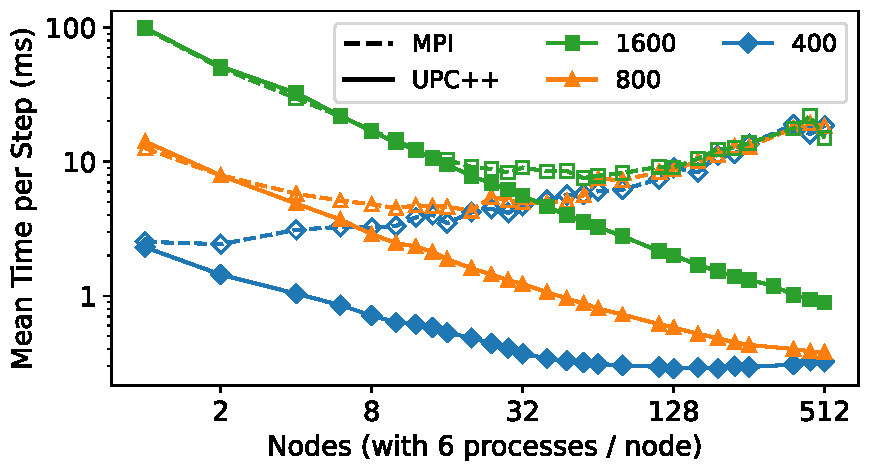
\includegraphics[width=0.72\textwidth]{projects/2.3.1-PMR/2.3.1.14-UPCxx-GASNet/paw21_interop_strong_scaling1.pdf}
  \caption{Mean run time per step (lower is better) in a strong scaling study
    comparing UPC++ (solid series) and MPI versions (dashed series) of a
    GPU-enabled 3D heat conduction example code, run on OLCF's Summit for three
    problem sizes (given as length of one edge of the cubic domain).}
  \label{fig:paw21_interop_strong_scaling}
\end{figure}


\paragraph{Recent Progress}

The most notable work in the past year has been in three areas:

\textbf{1. Memory Kinds.}
UPC++ ``memory kinds'' provide a unified abstraction for communication between
combinations of device (e.g. GPU) and host memory, possibly remote.  By
unifying the expression of data transfer among the various memories in a
heterogeneous system, these abstractions enable ECP
applications to utilize accelerators within UPC++'s PGAS model.  The
abstraction enables hardware offload (when available) of device data transfers,
eliminating the need for the application to stage transfers through
intermediate buffers in host memory.
The global pointer representation transparently tracks device information,
eliminating the need for expensive address space queries in critical paths.
Support for such offload on the OLCF's
Summit was initially demonstrated in October 2020, and subsequent releases
have hardened and tuned the implementation.

\textbf{2. Training and Outreach.}
The UPC++ team continues outreach efforts, including a half-day UPC++
tutorial to appear at SC21 (for the second consecutive year).

\textbf{3. Productivity and Performance.}
Having completed the core specification and implementation of UPC++, we have
shifted focus toward addressing improvements to productivity and performance,
especially in response to stakeholder feedback.  The most significant
examples are deployment of eager notification~\cite{pawatm21-upcxx-as_eager} 
and instruction-level tuning along common critical paths.

\paragraph{Next Steps}

The planned work for the near-term future includes the following:

\textbf{1. Memory Kinds.}
We will continue development of memory kinds.  The
implementation, currently targeting the hardware in Summit, will be extended to
include other accelerators scheduled to appear in early exascale systems.
As with Summit, transfers will be offloaded to available hardware capabilities
by leveraging the parallel efforts in GASNet-EX.

\textbf{2. Productivity and Performance.}
With the help of our stakeholders, we will continue to identify and address
portions of UPC++ where performance tuning is most needed
and/or beneficial.  Similarly, we will continue to work with stakeholders to
identify and implement features which improve productivity.

\textbf{3. Outreach.}
We will continue to engage with our users, such as by circulation of working
group drafts of new features to solicit feedback.
